%latex model.tex
%bibtex model
%latex model.tex
%latex model.tex
%dvipdfm model.dvi

%se poate lucra si online (de ex www.overleaf.com)


\documentclass[runningheads,a4paper,11pt]{report}

\usepackage{algorithmic}
\usepackage{algorithm} 
\usepackage{array}
\usepackage{amsmath}
\usepackage{amsfonts}
\usepackage{amssymb}
\usepackage{amsthm}
\usepackage{caption}
\usepackage{comment} 
\usepackage{epsfig} 
\usepackage{fancyhdr}
\usepackage[T1]{fontenc}
\usepackage{geometry} 
\usepackage{graphicx}
\usepackage[colorlinks]{hyperref} 
\usepackage[latin1]{inputenc}
\usepackage{multicol}
\usepackage{multirow} 
\usepackage{rotating}
\usepackage{setspace}
\usepackage{subfigure}
\usepackage{url}
\usepackage{verbatim}
\usepackage{xcolor}

\geometry{a4paper,top=3cm,left=2cm,right=2cm,bottom=3cm}

\pagestyle{fancy}
\fancyhf{}
\fancyhead[LE,RO]{MOE}
\fancyhead[RE,LO]{Raicu Robert}
\fancyfoot[RE,LO]{MIRPR 2019-2020}
\fancyfoot[LE,RO]{\thepage}

\renewcommand{\headrulewidth}{2pt}
\renewcommand{\footrulewidth}{1pt}
\renewcommand{\headrule}{\hbox to\headwidth{%
  \color{lime}\leaders\hrule height \headrulewidth\hfill}}
\renewcommand{\footrule}{\hbox to\headwidth{%
  \color{lime}\leaders\hrule height \footrulewidth\hfill}}

\hypersetup{
pdftitle={artTitle},
pdfauthor={name},
pdfkeywords={pdf, latex, tex, ps2pdf, dvipdfm, pdflatex},
bookmarksnumbered,
pdfstartview={FitH},
urlcolor=cyan,
colorlinks=true,
linkcolor=red,
citecolor=green,
}
% \pagestyle{plain}

\setcounter{secnumdepth}{3}
\setcounter{tocdepth}{3}

\linespread{1}

% \pagestyle{myheadings}

\makeindex


\begin{document}

\begin{titlepage}
\sloppy
\begin{center}
BABE\c S BOLYAI UNIVERSITY, CLUJ NAPOCA, ROM\^ ANIA

FACULTY OF MATHEMATICS AND COMPUTER SCIENCE

\vspace{6cm}

\Huge \textbf{MOE: classroom assistant}

\vspace{1cm}

\normalsize -- MIRPR report --

\end{center}


\vspace{5cm}

\begin{flushright}
\Large{\textbf{Team members}}\\
Raicu Robert, Software Engineering, 258/2
\end{flushright}

\vspace{4cm}

\begin{center}
2019
\end{center}

\end{titlepage}

\pagenumbering{gobble}

\begin{abstract}

    Working with young pupils is not easy, any teacher can tell you that. It's a period of life when they still develop and sometimes get easily discouraged or distracted especially when working on computers. Because of this, there is a need for classroom tools to allow only certain applications and monitor the emotional state of children as one teacher cannot keep track of an entire class at once.
    During this paper we will discuss the implementation of such an application using existing neural networks like FaceNet MTCNN \cite{SchroffKP15} for face detection, ResNet50  \cite{HeZRS15} for facial authentication and VGG16 \cite{VGG} for emotion recognition toghether with an .Net WPF application for the management of the classroom, applications, sessions and recordings.

    This paper is about the integration of multiple technologies and existing AI papers to create a useful application for managing the classroom, not about building or the optimizations of specialized neural networks. 
\end{abstract}


\tableofcontents

\newpage

\listoftables
\listoffigures
\listofalgorithms

\newpage

\setstretch{1.5}



\newpage

\pagenumbering{arabic}


 


\chapter{Introduction}
\label{chapter:introduction}

\section{What? Why? How?}
\label{section:what}

Young pupils have the tendency to be distracted or get demotivated easily while doing tasks in the classroom. Monitoring their emotions in relation to the task at hand can help us better understand when and why it happens. This allows the teachers to get insights on their behaviour and be able to restructure lessons or give personalized assistance to each pupil in order to maximize the information passed.
Our approach is to have a specialized application that allows the teacher to manage pupils, allowed apps and session recordings on which children can be logged in and out using facial recognition for ease of use.

\section{Paper structure and original contribution(s)}
\label{section:structure}

The research presented in this paper advances the design, combination and implementation of and application using particular models and technologies. 

The main contribution of this report is to present an intelligent solution for solving the problem of identifying how emotions can affect a classroom's productivity.

The second contribution of this report consists of building an intuitive, easy-to-use and user
friendly software application. Our aim is to build an application that requires no teacher interaction while pupils use it such that he/she can concentrate on other tasks.

The present work contains 7 bibliographical references and is structured in five chapters as follows.

The first chapter/section is a short introduction.

The second chapter/section describes the problem the paper wants to solve.

The third chapter/section talks about related work in the field.

The chapter/section \ref{chapter:proposedApproach} describes the proposed approach.

The fifth chapter/section talks about the implementation of the model used.

The sixth chapter/section presents the conclusion.


\chapter{Scientific Problem}
\label{section:scientificProblem}


\section{Problem definition}
\label{section:problemDefinition}
The goal of our application is to help teachers track the pupils emotional state during the use of computers in didactic activities in order to better understand their behaviour. The need for an automated solution like this comes from the sheer amount of information and subjects. A single person would not be able to perform their didactic activities while also monitoring the current activity and facial expression of each pupil in a full classroom.

As we know, face recognition is nothing new as it started in the years 1964-1968 \cite{Bledsoe} where facial features were mapped by hand. A huge breakthrough came when in the early 2000's the process was automated using AI. Since then many advancements the field of face recognition and mapping were made using state of the art topologies.

For this task we used three neural networks:  ResNet \cite{HeZRS15} and VGG \cite{VGG} from the Keras \cite{Ker} library in Tensorflow \cite{Tf} and a FaceNet MTCNN \cite{SchroffKP15} implementation.

\section{FaceNet MTCNN I/O}
\label{section:faceNetMTCNNI/O}
FaceNet \cite{SchroffKP15} is used in order to crop the face if the pupil from a raw camera image.
The input image can be any size although the performance will be impacted. 
The output that we are interested in is an array of bounding boxes that represent detected faces.

\section{ResNet I/O}
\label{section:resNetI/O}
ResNet \cite{HeZRS15} is used in order to extract facial features in the cropped image such that we can identify individuals. The netural network was pre-trained on the ImageNet dataset.
The input image has to be 224x224 pixels having three color channels.
The output is a 2048 array of doubles that represent the facial features of the subject.


\section{VGG I/O}
\label{section:vGGI/O}
VGG \cite{VGG} is used in order to recognize the emotion of the pupil. In order to do this, the VGG16 architecture is used without the top layer leaving a 512 double array base output. From this, a model is appended to map the 512 output to a 7 class output (Angry, Disgust, Fear, Happy, Sad, Surprise, Neutral). Then the model is trained on the Fer2013 image set.

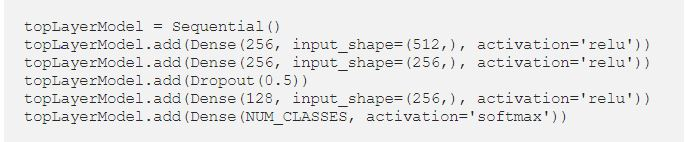
\includegraphics[width=\linewidth]{./Fig/EmotionLayers.JPG}

The input of the model will is 43x43 pixels with tree color channels. The issue is that the Fer2013 image set is grayscale and because of this the cropped image of the face has to be converted to grayscale then used as an input of all three channels. 

\chapter{State of art/Related work}
\label{chapter:stateOfArt}

One example of a paper on this subject is "Deep Learning based Student Emotion Recognition from Facial Expressions in Classrooms" \cite{DLSEC}. It proposes a system where two high resolution cameras are positioned in front of a classroom and record all emotions in order for teachers to improve their lectures such that students pay attention. The main difference in between the system described by the cited paper and the one implemented here is that theirs take a group approach as an emotion metric and it's concentrated on the emotion as a group where our approach is centered around the individual.


\chapter{Proposed approach}
\label{chapter:proposedApproach}

In order to create such a application we need to solve 4 sub-problems:
\begin{itemize}
  \item detect and crop the the face of the subject from the image
  \item create a form of identification for the given face
  \item identify the emotion expressed by the subject
  \item create a application to serve as an interface for the pupils and the teacher
\end{itemize}

After solving these problems using the neural networks described in chapter 2 and using the .Net framework we can implement the application described in the following sections.

\pagebreak
\section{Overall architecture}
\label{section:overallArchitecture}

The application is split into 2 main parts and a communication channel. This was designed this way because of the nature of the machine learning libraries as they run on the Python platform. 

The communication channel is represented by the GRPC library created by Google that uses protocol buffers in order to transmit data between services. Because of this we can make remote procedure calls between Python and C\# with little effort so we can transfer the necessary data with a low overhead.

The first part is the Python server which is responsible for the image processing. It handles image capture, face cropping, emotion detection and face features extraction. This data is bundled and sent through the GRPC library to the main application to be used.

The second part is the .Net application called "MOE" which is responsible for managing applications, pupils, sessions and authentication. This application is where all business logic and user interaction layer resides.

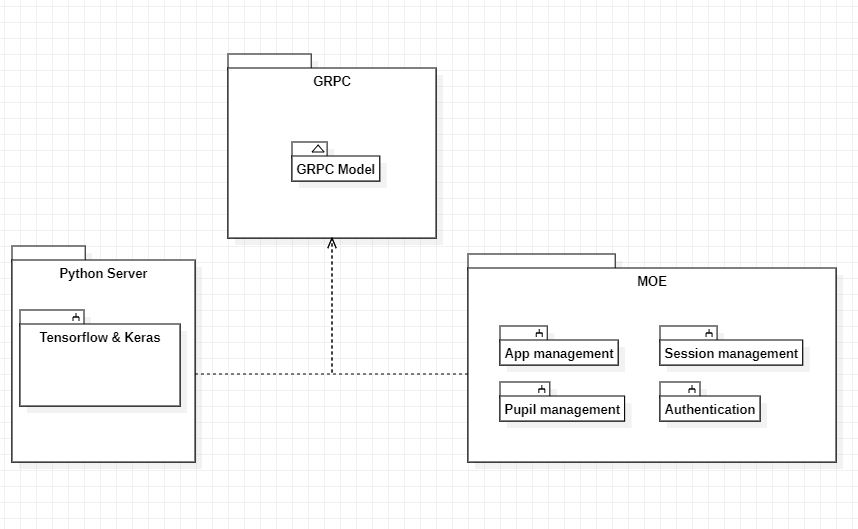
\includegraphics[width=\linewidth]{./Fig/OverallArchitecture.JPG}

\pagebreak
\section{Python server}
\label{section:pythonServer}

The Python server serves as the visual processing hub. Using CV2 it captures live video frames and processes them using Tensorflow and Keras in order to extract the required information.
The captured image is 1280x720 pixels and is fed to the FaceNet MTCNN model which in turn returns a bounding box if a face is found. Then we cut the face from the original frame and using ResNet we calculate the face embedding whitch we use as a form of identification. From the original frame we also pre-process a grayscale image that we feed to the VGG composed model such that we can extract the emotion. 

The final process is that we pack the cropped image, the emotion and face embedding in a message and send it to the .Net application using GRPC to be used.

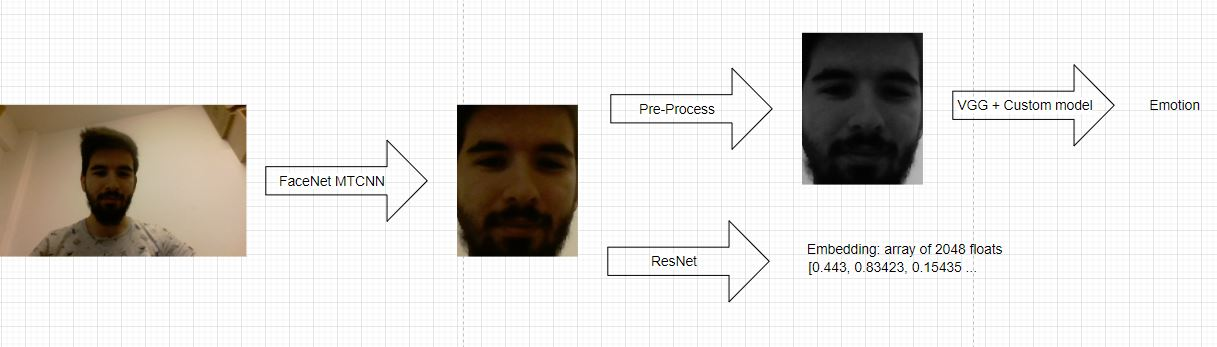
\includegraphics[width=\linewidth]{./Fig/FacePipeline.JPG}

\pagebreak
\section{.Net application}
\label{section:pythonServer}

The .Net application serves as the 'brains' of the operation. It manages all aspects starting from database connection to business logic and user interaction.
The application is split into two parts: the managing side for the teacher and the desktop side for the pupils.

The managing side of the application offers 3 services
\begin{itemize}
    \item the management of registered applications
    \item the management of registered pupils
    \item a history of recorded sessions.
\end{itemize}

On the "Apps" screen the teacher can configure which applications can be used by the pupils in the class. Applications can be added or removed using the "+" or "X" icons on the screen. Only applications previously configured by the teacher will be available to the students.
\newline
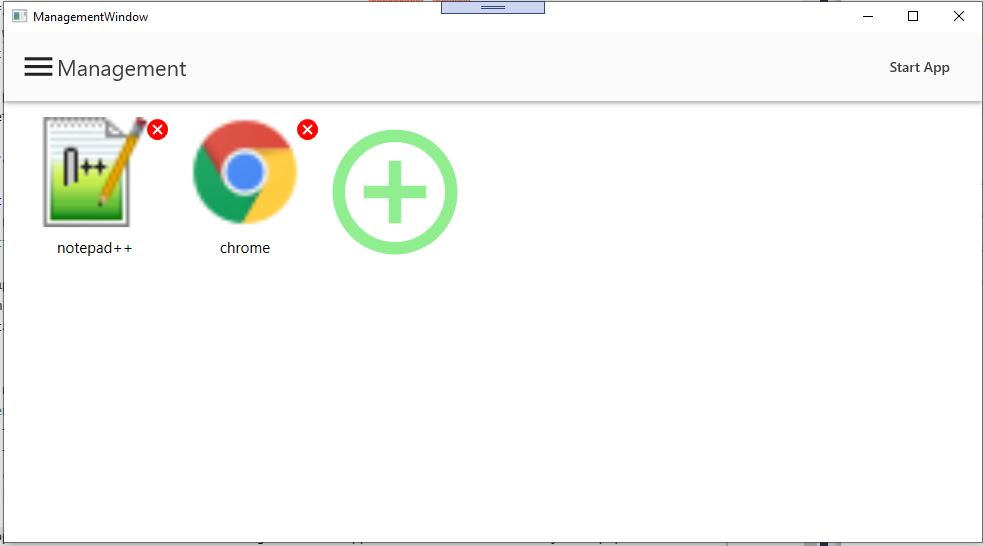
\includegraphics[width=0.5\linewidth]{./Fig/Apps.JPG}

On the "Students" screen the teacher can manage the pupils that can access the system. Students can be added or removed using the "+" or "X" icons on the screen. Only students previously added by the teacher will be available to login into the application.
\newline
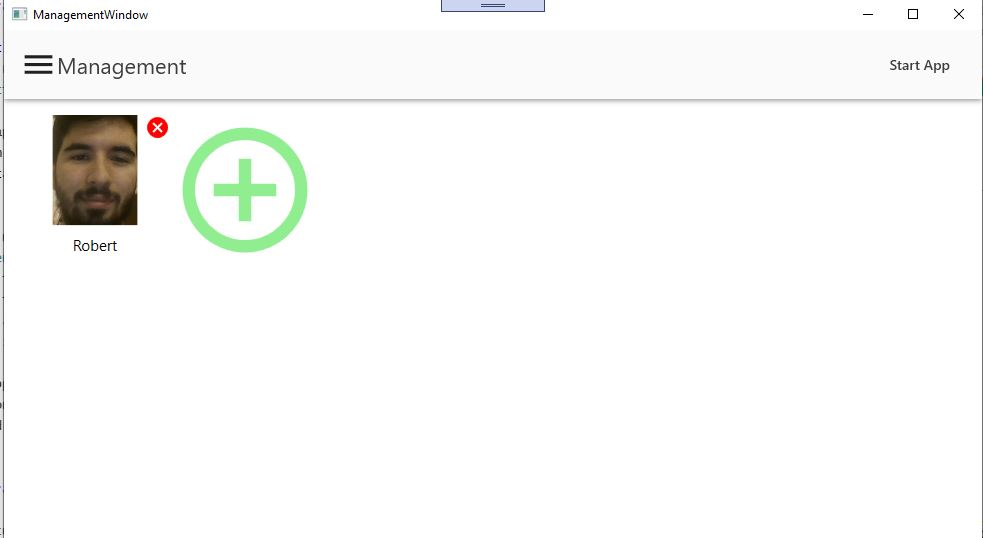
\includegraphics[width=0.5\linewidth]{./Fig/Students.JPG}

\pagebreak
On the "Sessions" screen the teacher and review previously recorded sessions. A session starts recording when a pupil opens an app and registers all emotions that he/she displays. The sessions ends when the pupil closes the application or logs out. On this screen the teacher can see when the session was recorded, which app was used an by which student. There are also two charts: one representing a timeline of the emotions displayed and one pie chart representing the percentage of time a certain emotion was displayed. All emotions are color coded and visible as a legend.
\newline
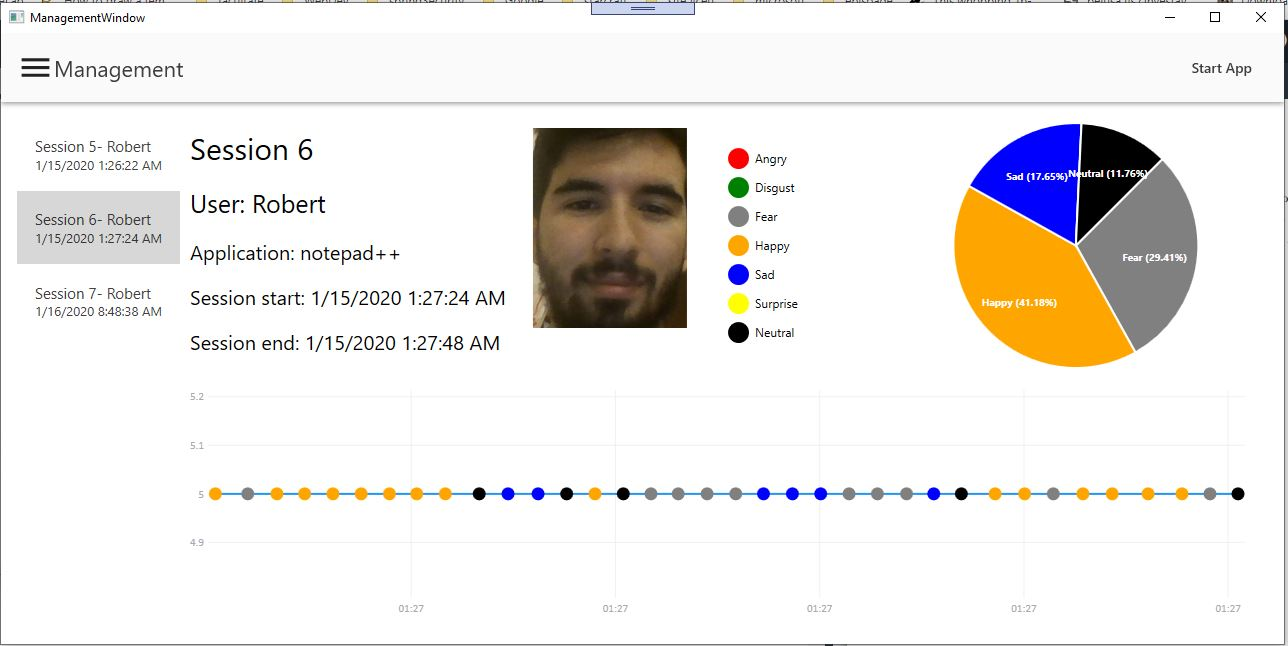
\includegraphics[width=0.5\linewidth]{./Fig/Sessions.JPG}

The desktop side of the application for the pupil has two important systems at play.

The first one is the authentication manager and login dialog. It uses the information provided by the python server to compare the recorded embedding to the ones registered by the teacher. If the same pupil is visible for a pre-configured amount of time, he/she will be logged in and the dialog will disappear. When the pupil leaves the camera's view, the system will countdown a pre-configured ammout of time before logging out the current user and showing the login dialog again.
\newline
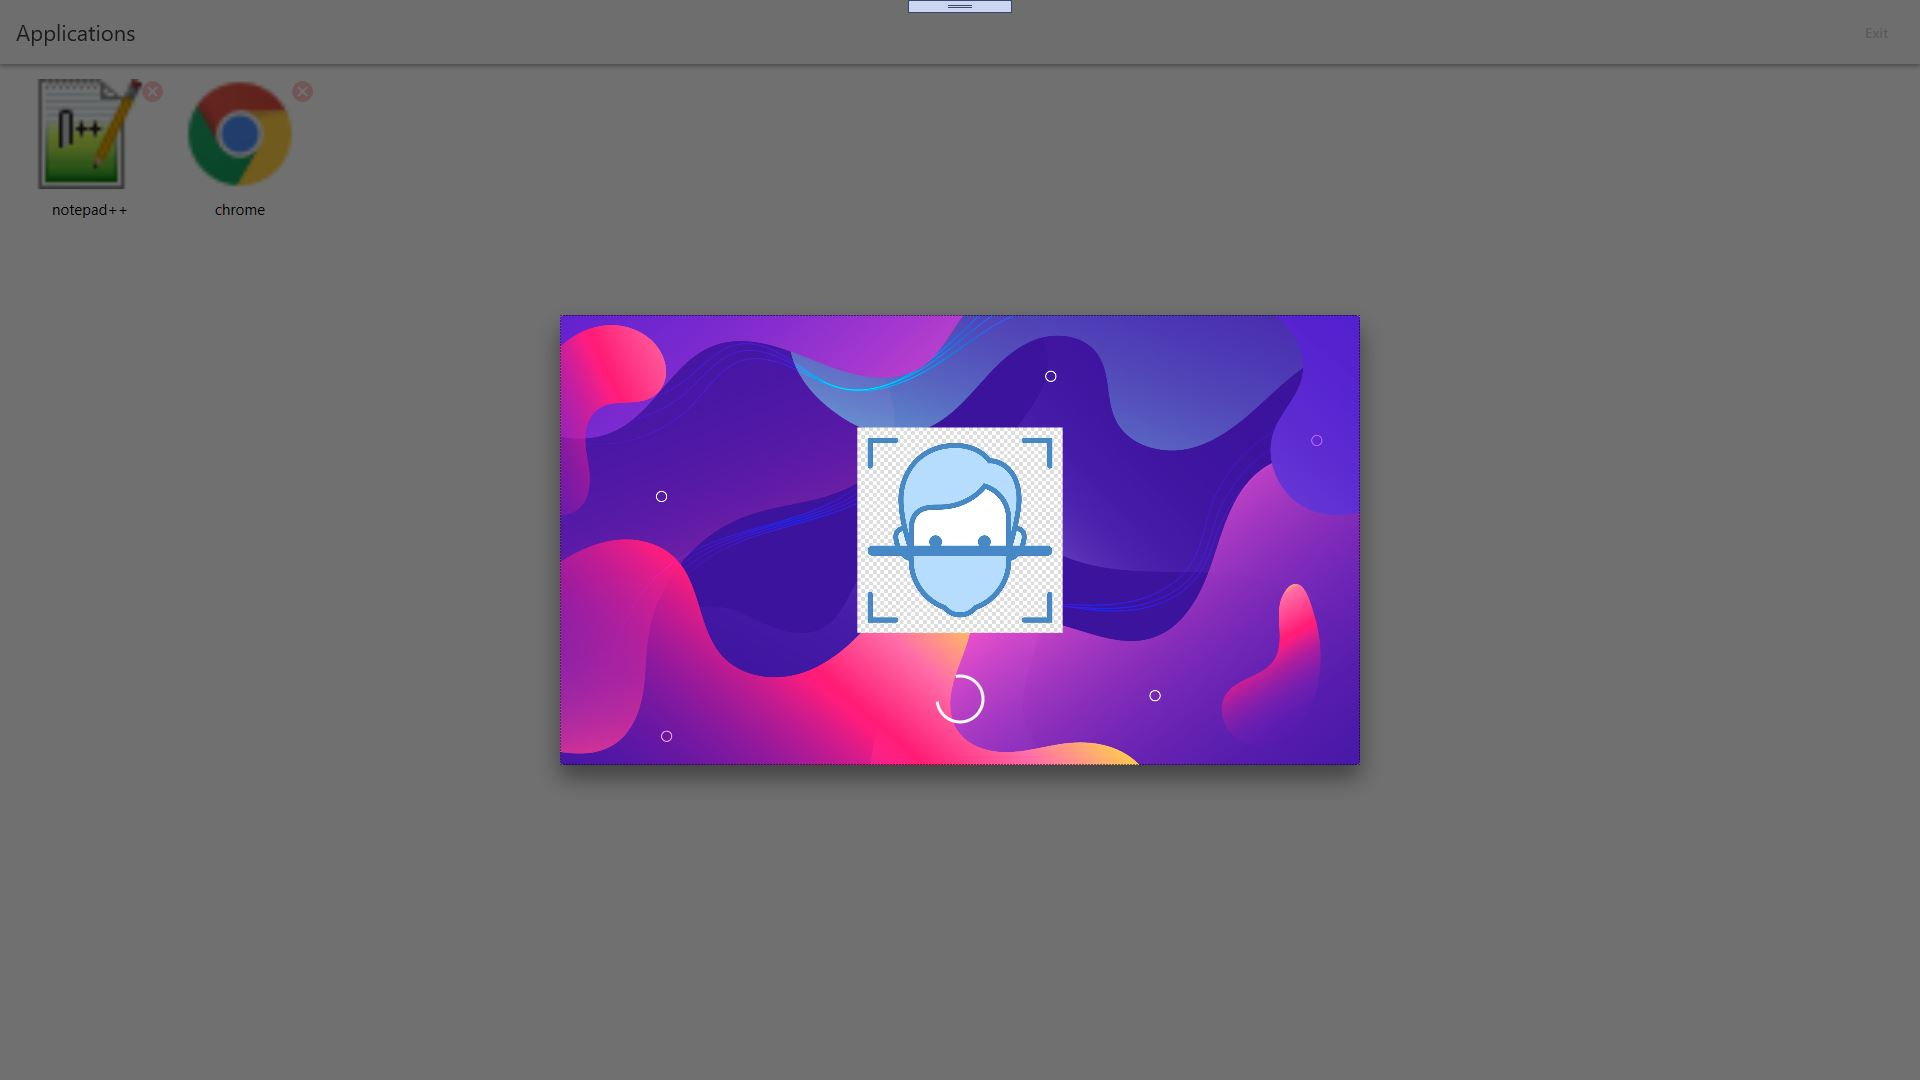
\includegraphics[width=0.5\linewidth]{./Fig/Login.JPG}

The second one is the session manager which is started when the pupil selects one of the available applications. This will start a session recording which takes the current user and the selected application and stores time and emotion data pairs in the database. When the pupil closes the application the recording is stopped

\chapter{Application (numerical validation)}
\label{chapter:application}

In this chapter we discuss discuss the model appended to VGG16 in order to detect the emotion of the user.

\section{Methodology}
\label{section:methodology}

\begin{itemize}
	\item As our emotion classification is essentially a classification problem, for evaluation we use precision and validation loss.
	\item The aim is to get better insights on the emotions pupils express during classes and test it's performance on real world data.
\end{itemize}

\section{Data}
\label{section:data}

As described earlier, we performed transfer-learning on the VGG16 architecture trained on the "ImageNet" set by combining it with our custom model and retraining on the "Fer2013" data set. The model attached to the VGG16 architecture is described in the image below.

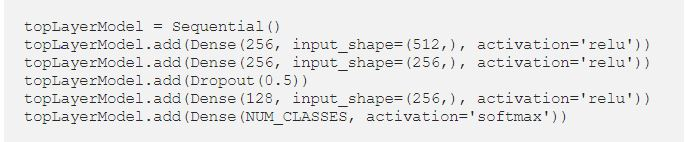
\includegraphics[width=\linewidth]{./Fig/EmotionLayers.JPG}

The VGG16 architecture was expecting a 3 color channel image so we had to use the grayscale image for each of the channels in order to train the network on the "Fer2013" data set.

\section{Results}
\label{section:results}

Using the model described above we managed to achieve the following accuracy:
\begin{itemize}
    \item training set (Model has seen these): 99.8%
    \item test/validation set (New inputs to model): 43.7
\end{itemize}

\section{Discussion}
\label{section:discussion}

Even if we did not reach state of the art results for emotion classification we believe that the application has real world application in education and research. Using custom models and better data sets could improve the results by a considerable margin. 

\chapter{Conclusion and future work}
\label{chapter:concl}

As we stated in the beginning our goal was not to improve or implement advanced neural networks but to show how important the integration of such technologies could prove in a real life scenario. 
The use of AI in day to day life is still new even though we came a long way in such a short time. Using tools like this can help us improve processes that were done only with human interaction until now.

\bibliographystyle{plain}
\bibliography{BibAll}

\end{document}
